\subsection{Projektstyring}


\subsection{Problemidentifikation}
Af de givne projektoplæg, har vi valgt at fokusere op det trejde projektoplæg (Når hdverdagen rystes), da dette ser ud til at være det mest spændende for os, da det passer ind i vores interesse og vores kompetencer.

%%%% PROBLEMIDENTIFIKATION FIG
\begin{figure}[H]
    \centering
    \fbox{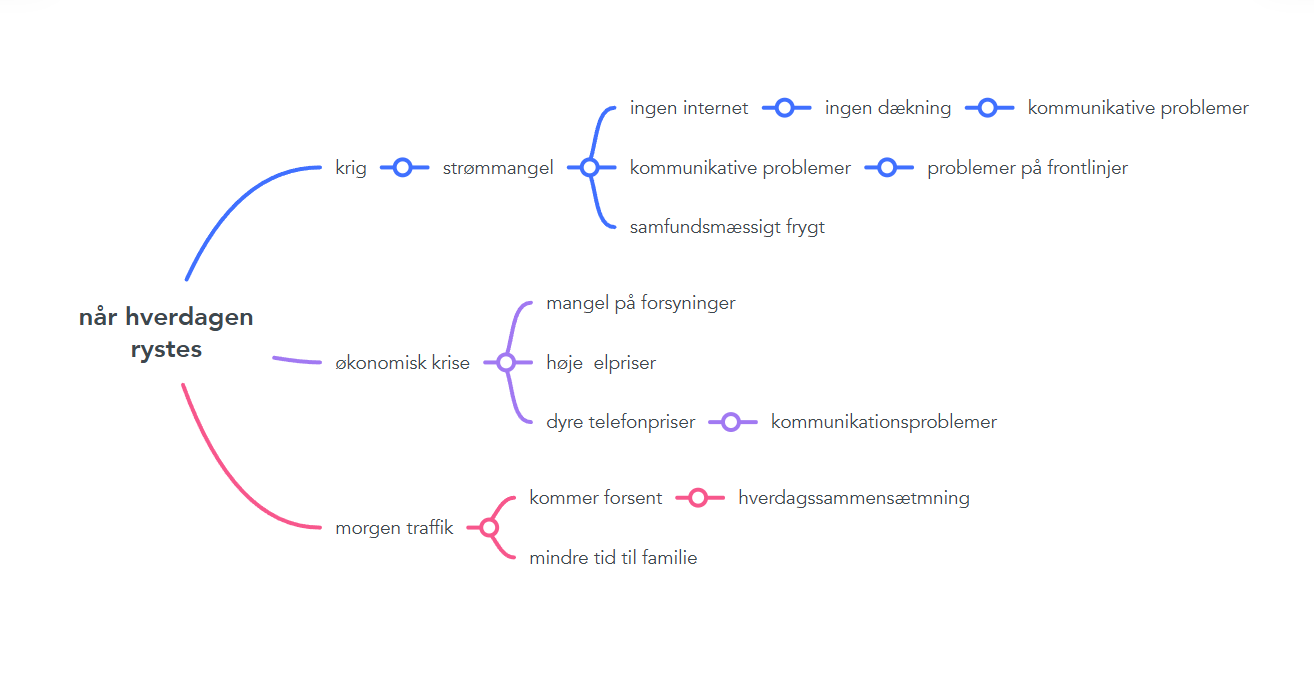
\includegraphics[width=\textwidth]{images/problem-identification.png}}
    \caption{Problemidentifikation}
\end{figure}


I dette projekt, har vi valgt at arbejde med den følgende problemstilling:

Efter ukrainekrigens udbrud i 2022, har verdensbilledet ændret sig markant, det ses bla. ved at beredskabsstyrelsen har lancerert helt kontrete retningslinjer til hvordan danskerne kan forberede sig til eventuelle krisesituationer, som kunne opstå. Hvis en af de krisesituationer, som beskrives i brredsskabssstyrelsens retningslinjer, skulle opstå må det siges at det ville have en stor inflydelse for alle danskernes liv, og heraf vil dette udgør en stor samfundsrelavans.

Vi har i gruppen valgt at opstille et problemtræ, hvilket er en af de teknologifaglige værktøjer, 
som vi kan bruge til at hjælpe med afgrænsningen af det som vi vil arbejde videre med. Problemtræet er endvidere en god måde, hvorpå vi i gruppen kan afprøve om det problem vi har valgt har nok som vi kan arbejde videre med. Problemtræet som ses på figur \ref{fig:problemtræ}, er opstillet således at i midten ses vores nøgleproblem, som udspæmder mod nord, virkningen af det pågældene nøgleproblem, og mod syd årsagerne til det samme.

%%%% PROBLEMTRÆ FIG
\begin{figure}[H]
    \centering
    \fbox{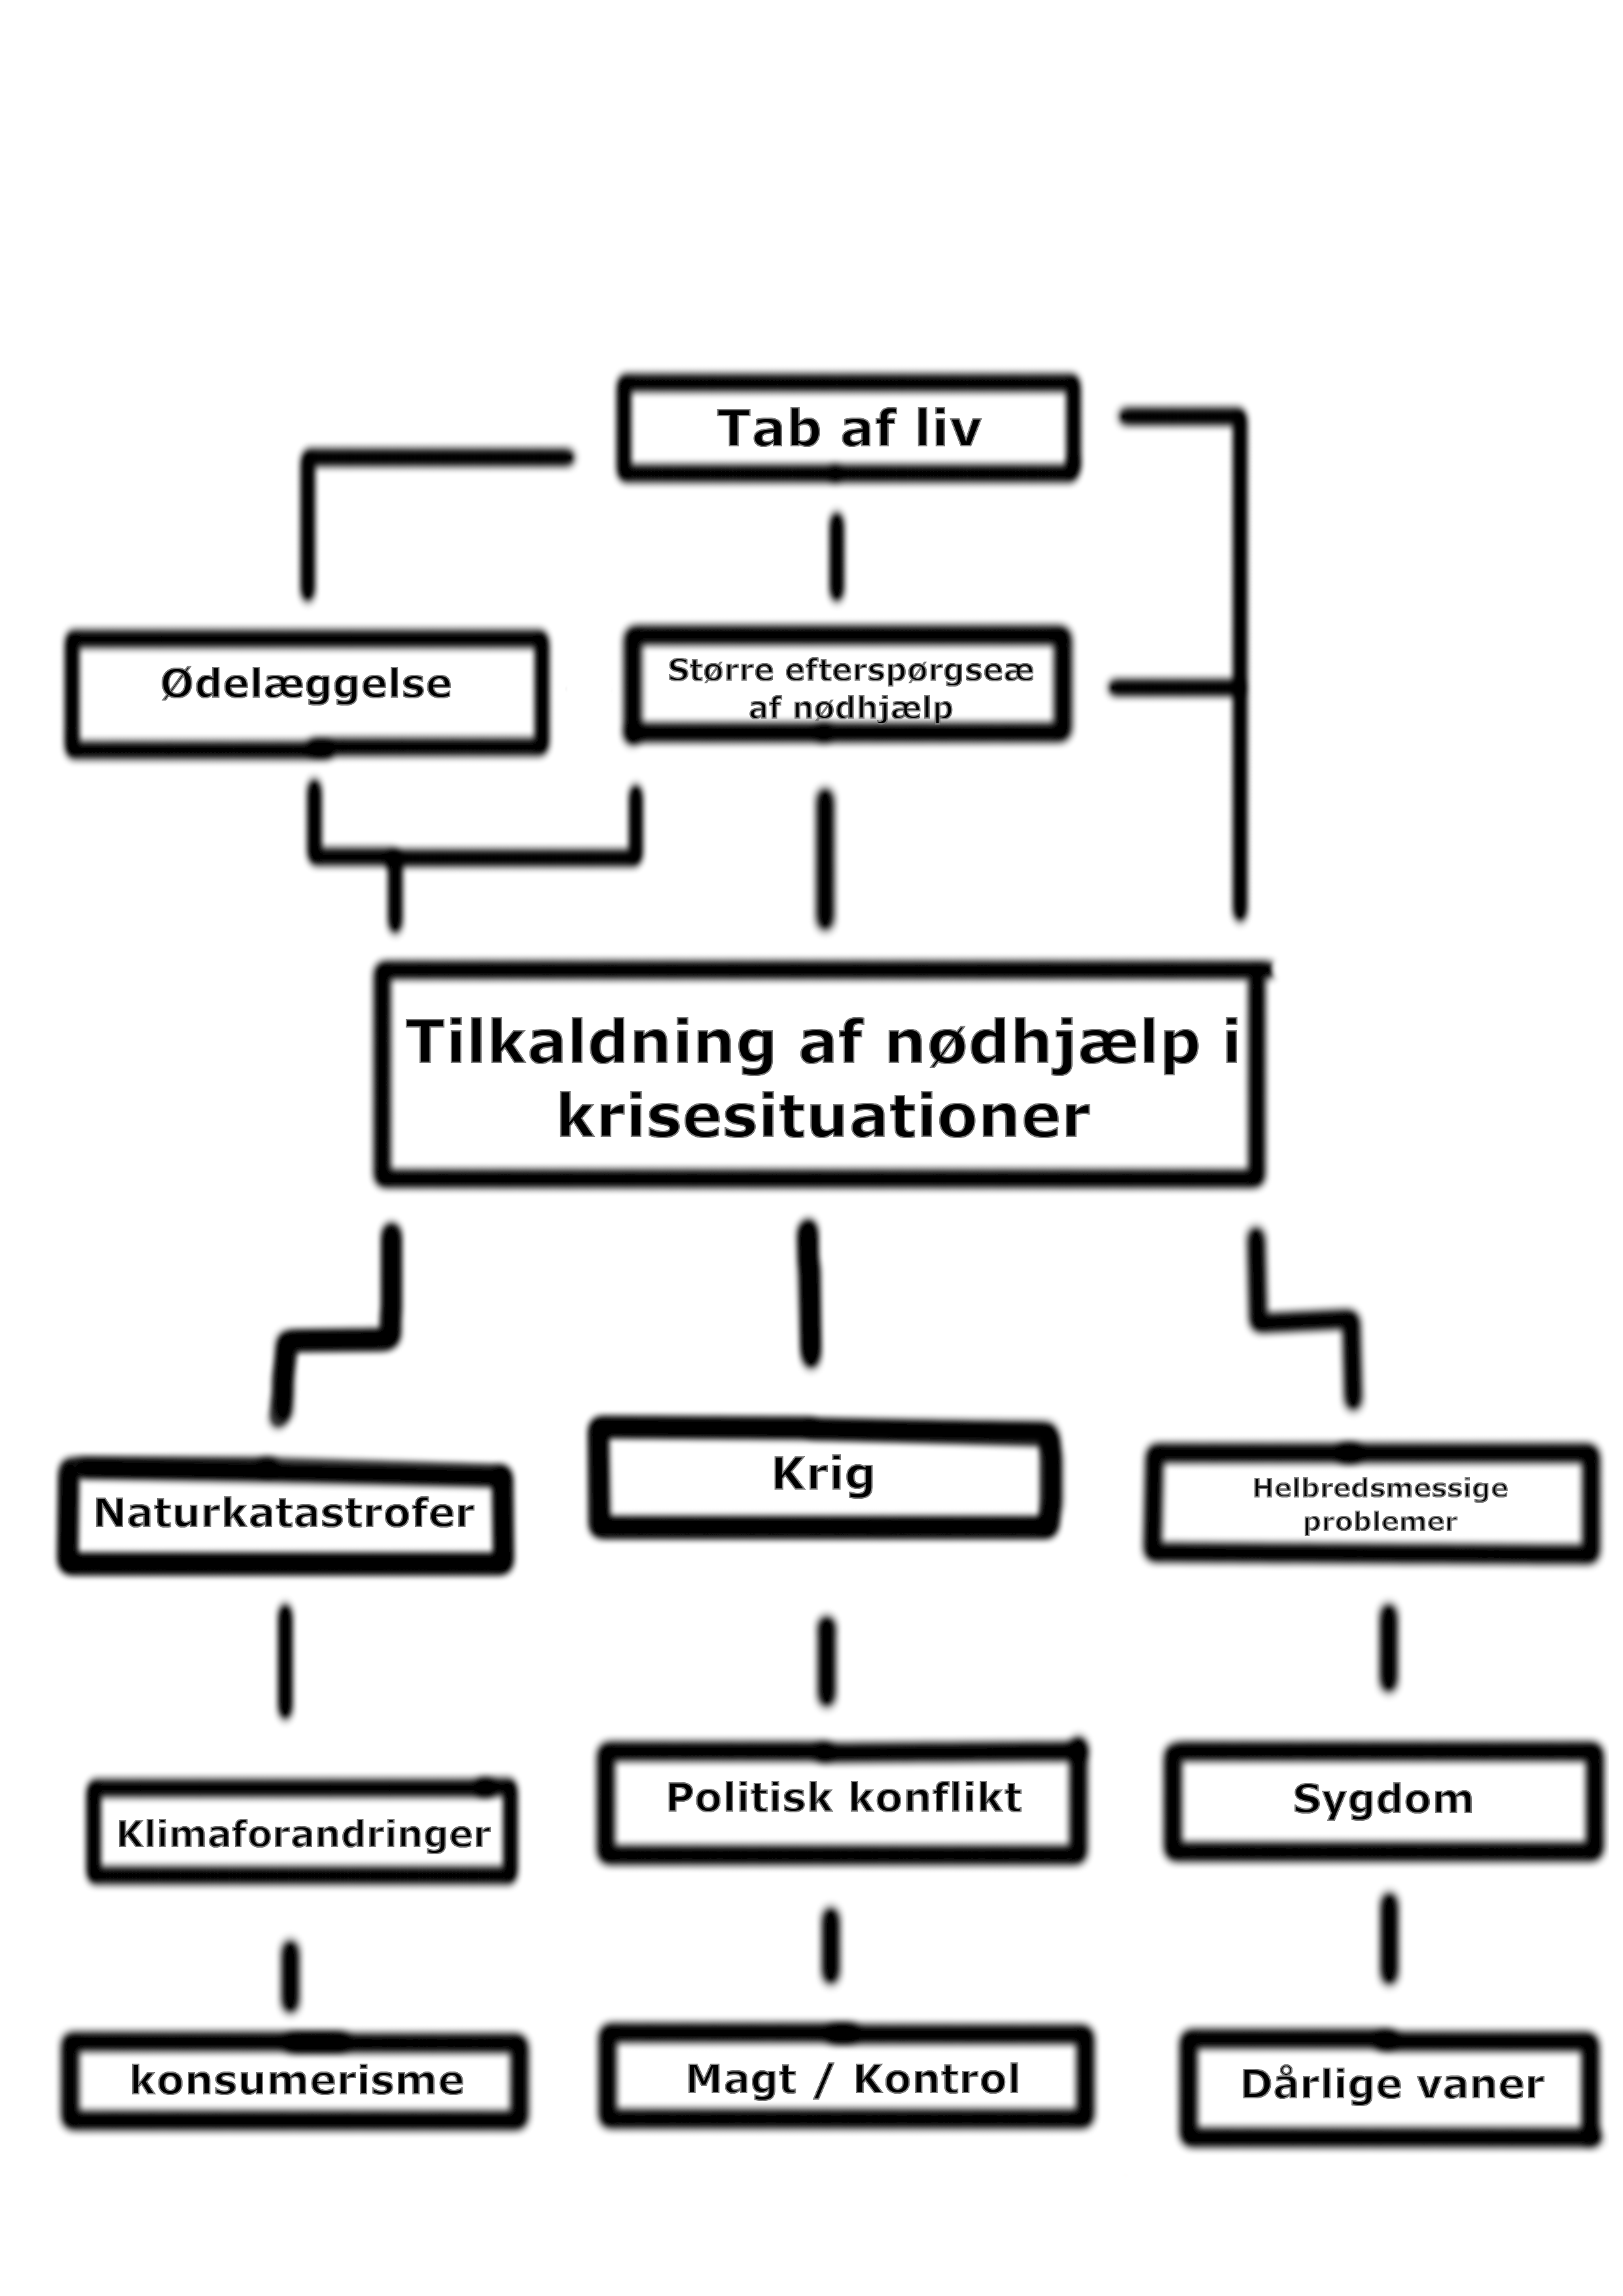
\includegraphics[width=0.6\textwidth]{images/rev_problemtree_no_OUT.png}}
    \label{fig:problemtræ}
    \caption{Problemtræ}
\end{figure}


\subsection{Lyskurven}
Lyskurven, er en metode, som kan benyttes til at sortere i de problemer, som vi har identificeret. Lyskurven funger således at de identificerede problemer, bliver placeret i 3 kategorier: Rød, Gul og Grøn. Disse betyder hhv. Rød, som er de problemer som vi vælger fra. Så er der gul, som er de problemer, som vi har vurderert til måske at kunne arbejde videre med, og som kan tages ibrug, hvis der ikke er nogle ideer som har fået grøn, eller hvis vi senere bliver nødt til at justere problemet. Til sidst er der grøn, som er de problemer, som vi har valgt at arbejde med.

\begin{table}[H]
\centering
\begin{tabular}{|p{0.3\textwidth}|p{0.6\textwidth}|}
\hline
\textbf{Kategori} & \textbf{Beskrivelse} \\
\hline
Rød & Mangel på forsyninger, Høje elpriser, Dyre telefonpriser, falske opkald, lommeopkald, mangel på server størrelse \\
\hline
Gul & blokering af signaler i krisesituation \\
\hline
Grøn & Tilkaldning af nødhjælp i krisesituationer \\
\hline
\end{tabular}
\caption{Lyskurve kategorier}
\label{tab:lyskurve}
\end{table}

\newpage
\subsection{Afgrænsning}
I denne teknologirapport har vi valgt at afgænse os til at se på hvordan man kan afhjælpe håndteringen af tildkaldelse af nødhjælp, under en krisesituation. Vi har valgt at bruge lyskurven (\ref{tab:lyskurve}) til at afgænse os til at arbejde med det grønne problem, som ses i Lyskurven (\ref{tab:lyskurve}). Herefter vises dette med en afgrænsning af problemtræet (\ref{fig:problemtræ}), som ses på figur (\ref{fig:afgrænsning}).
 
\begin{figure}[H]
    \centering
    \fbox{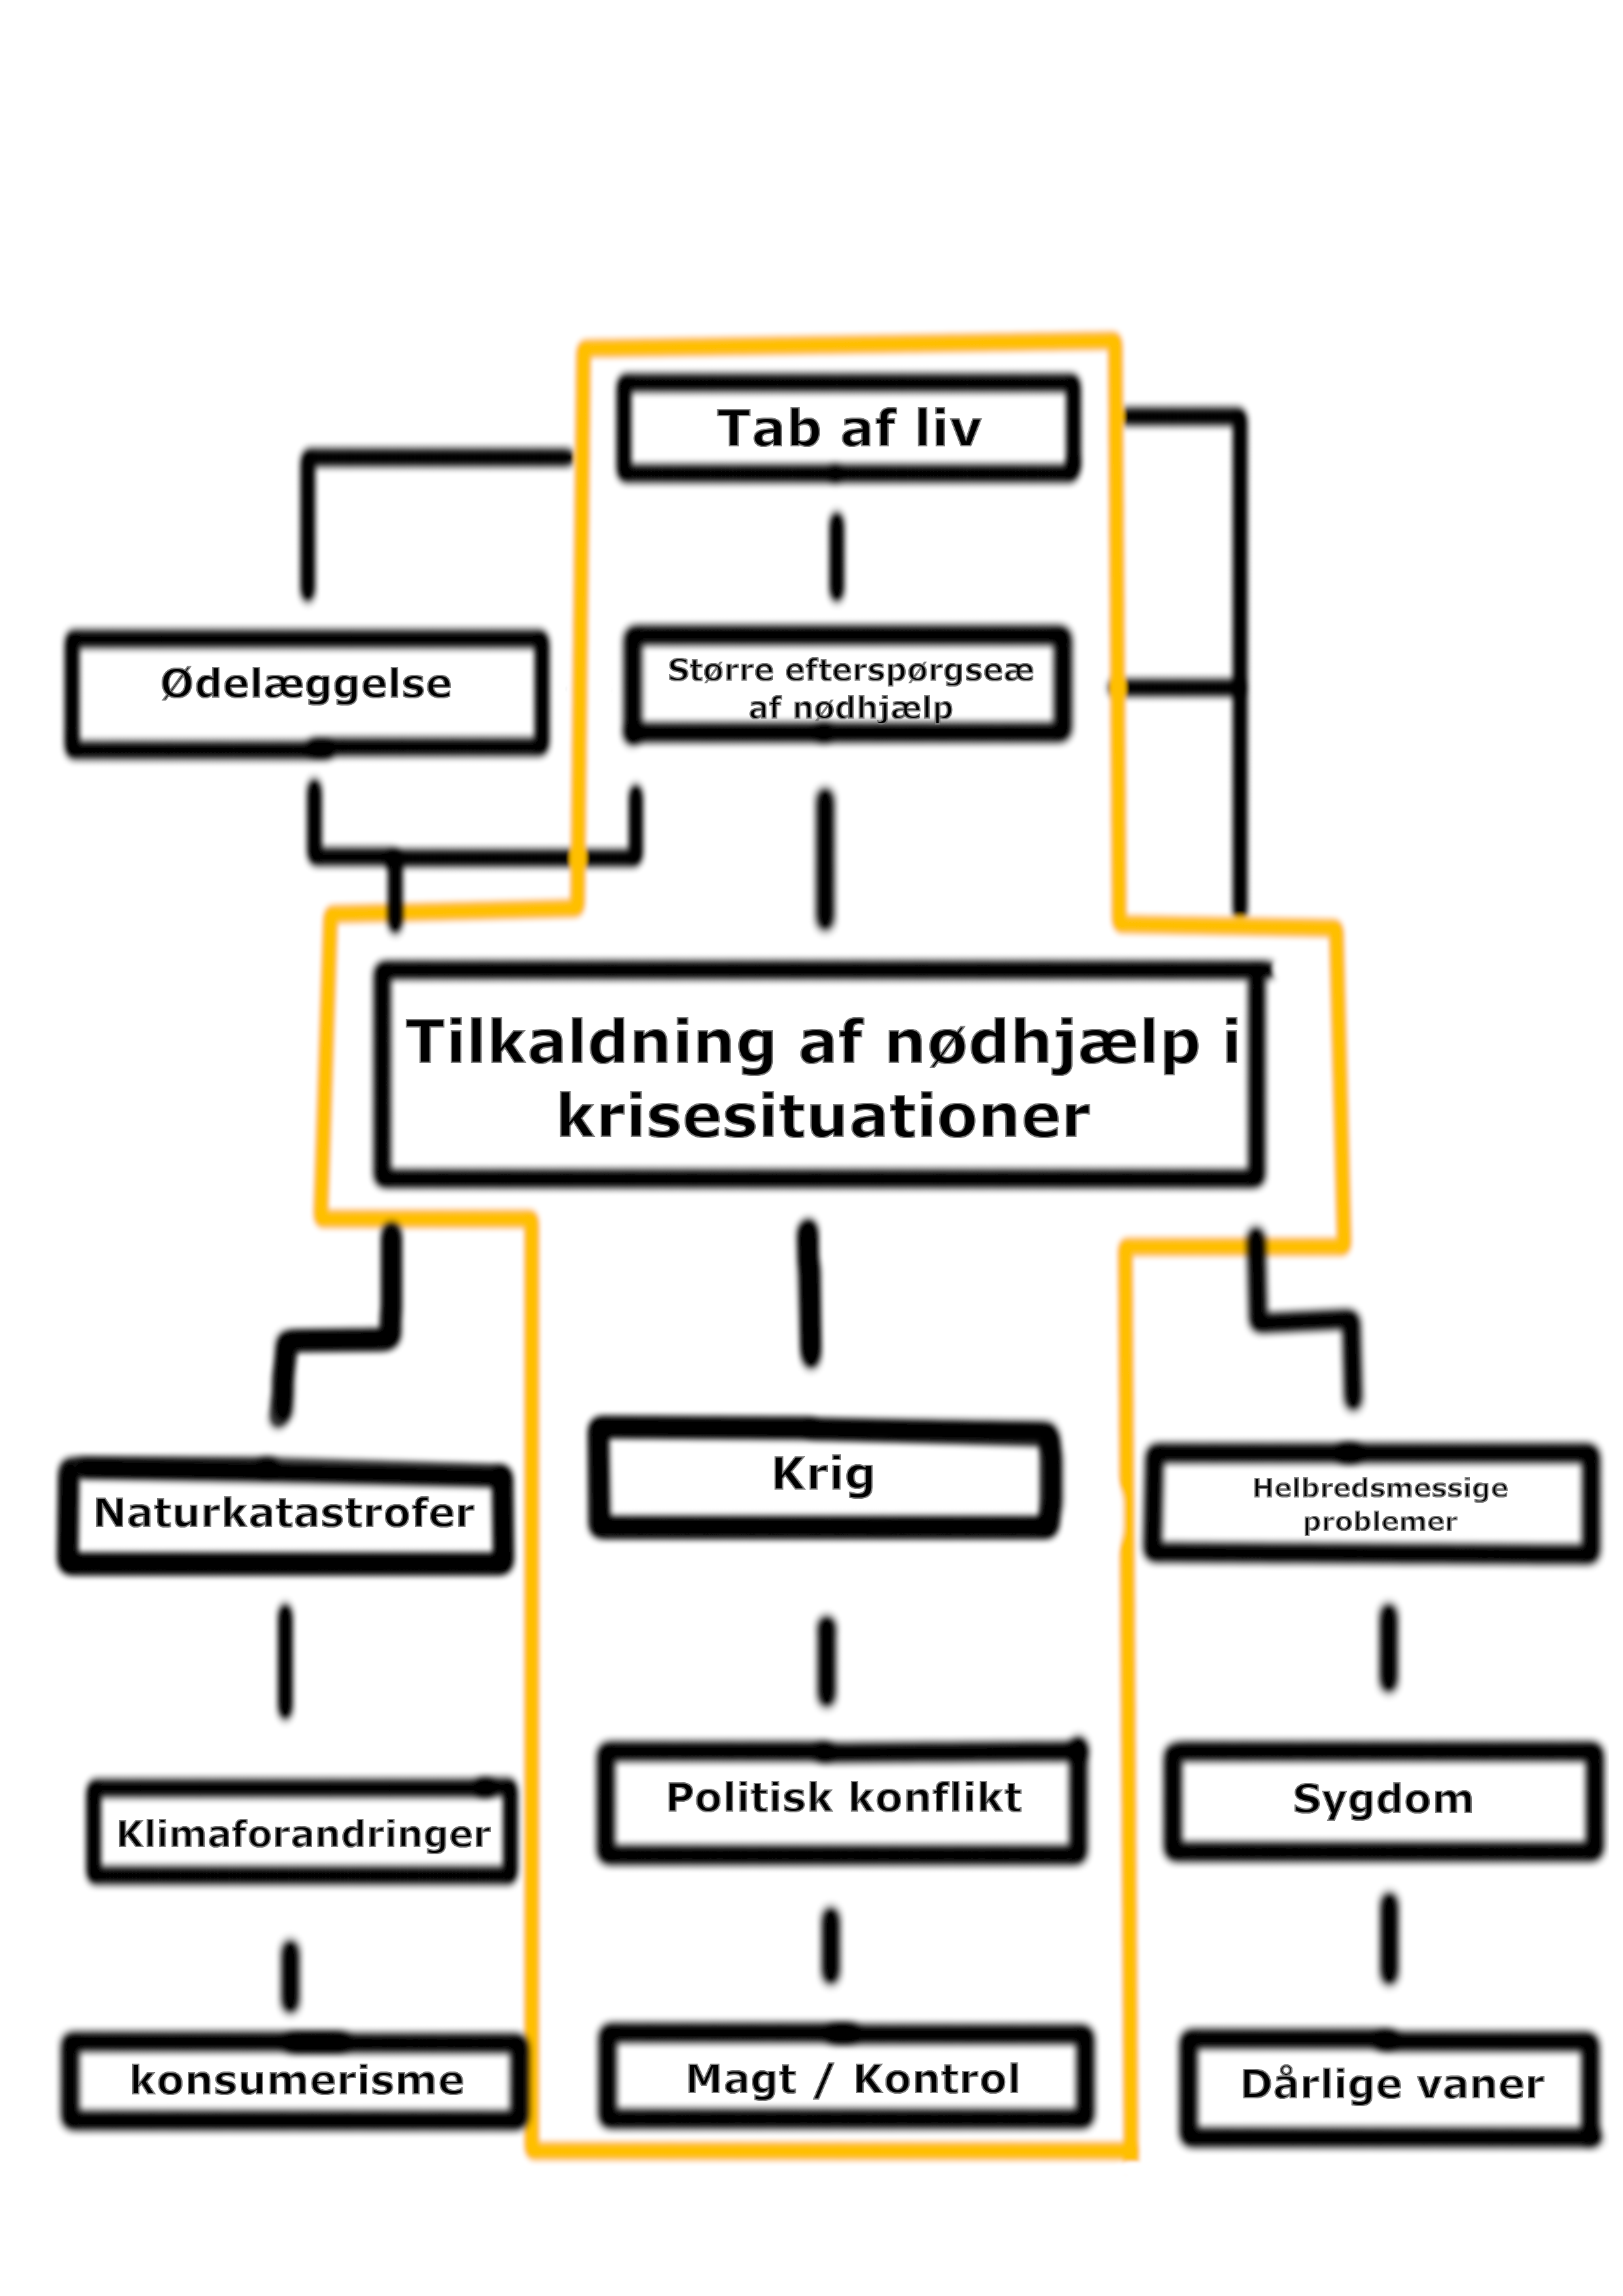
\includegraphics[width=0.6\textwidth]{images/rev_problemtree_OUT.png}}
    \caption{Afgrænsning}
    \label{fig:afgrænsning}
\end{figure}